%!TeX root=../pridetop.tex

\chapter[Chapter \thechapter]{}
\begin{figure}[t!]
\centering
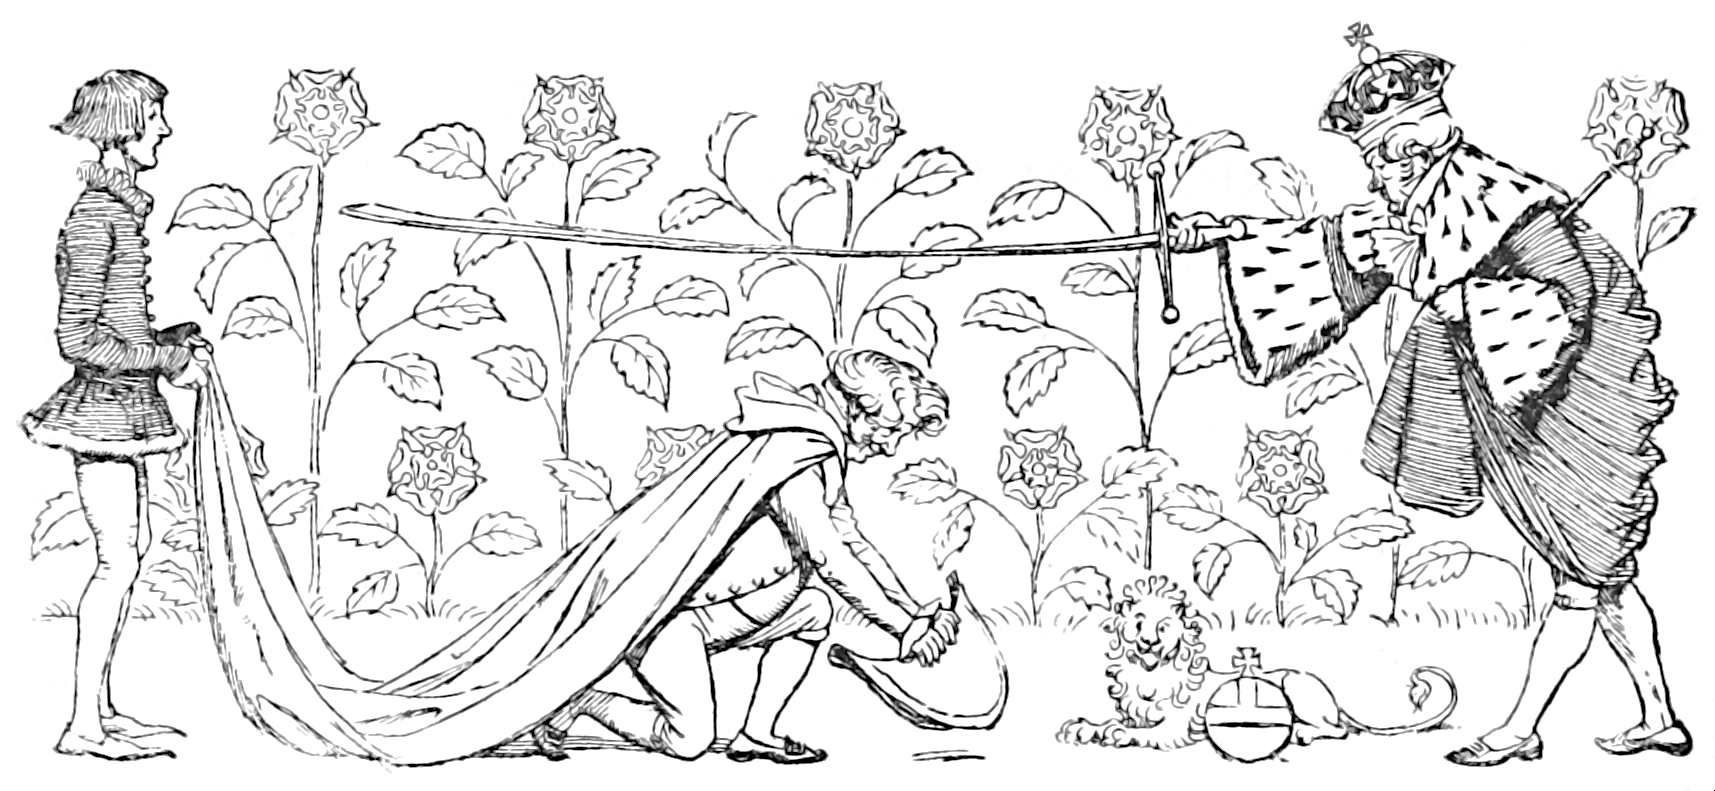
\includegraphics[width=\linewidth]{5top}
\captionlistentry{Headpiece to Chapter \thechapter}
\end{figure}

\lettrine[lines=6,image=true]{initials/chap5w}{ithin}  a short walk of Longbourn lived a family with whom the Bennets were particularly intimate. Sir William Lucas had been formerly in trade in Meryton, where he had made a tolerable fortune, and risen to the honour of knighthood by an address to the king during his mayoralty. The distinction had, perhaps, been felt too strongly. It had given him a disgust to his business and to his residence in a small market town; and, quitting them both, he had removed with his family to a house about a mile from Meryton, denominated from that period Lucas Lodge; where he could think with pleasure of his own importance, and, unshackled by business, occupy himself solely in being civil to all the world. For, though elated by his rank, it did not render him supercilious; on the contrary, he was all attention to everybody. By nature inoffensive, friendly, and obliging, his presentation at St James's had made him courteous.

Lady Lucas was a very good kind of woman, not too clever to be a valuable neighbour to Mrs Bennet. They had several children. The eldest of them, a sensible, intelligent young woman, about twenty-seven, was Elizabeth's intimate friend.

That the Miss Lucases and the Miss Bennets should meet to talk over a ball was absolutely necessary; and the morning after the assembly brought the former to Longbourn to hear and to communicate.

»\textit{You} began the evening well, Charlotte,« said Mrs Bennet, with civil self-command, to Miss Lucas. »\textit{You} were Mr Bingley's first choice.«

»Yes; but he seemed to like his second better.«

»Oh, you mean Jane, I suppose, because he danced with her twice. To be sure that \textit{did} seem as if he admired her—indeed, I rather believe he \textit{did}—I heard something about it—but I hardly know what—something about Mr Robinson.«

»Perhaps you mean what I overheard between him and Mr Robinson: did not I mention it to you? Mr Robinson's asking him how he liked our Meryton assemblies, and whether he did not think there were a great many pretty women in the room, and \textit{which} he thought the prettiest? and his answering immediately to the last question, »Oh, the eldest Miss Bennet, beyond a doubt: there cannot be two opinions on that point.««

»Upon my word! Well, that was very decided, indeed—that does seem as if—but, however, it may all come to nothing, you know.«

»\textit{My} overhearings were more to the purpose than \textit{yours}, Eliza,« said Charlotte. »Mr Darcy is not so well worth listening to as his friend, is he? Poor Eliza! to be only just \textit{tolerable}.«

»I beg you will not put it into Lizzy's head to be vexed by his ill-treatment, for he is such a disagreeable man that it would be quite a misfortune to be liked by him. Mrs Long told me last night that he sat close to her for half an hour without once opening his lips.«

\begin{figure}[tbh!]
\centering
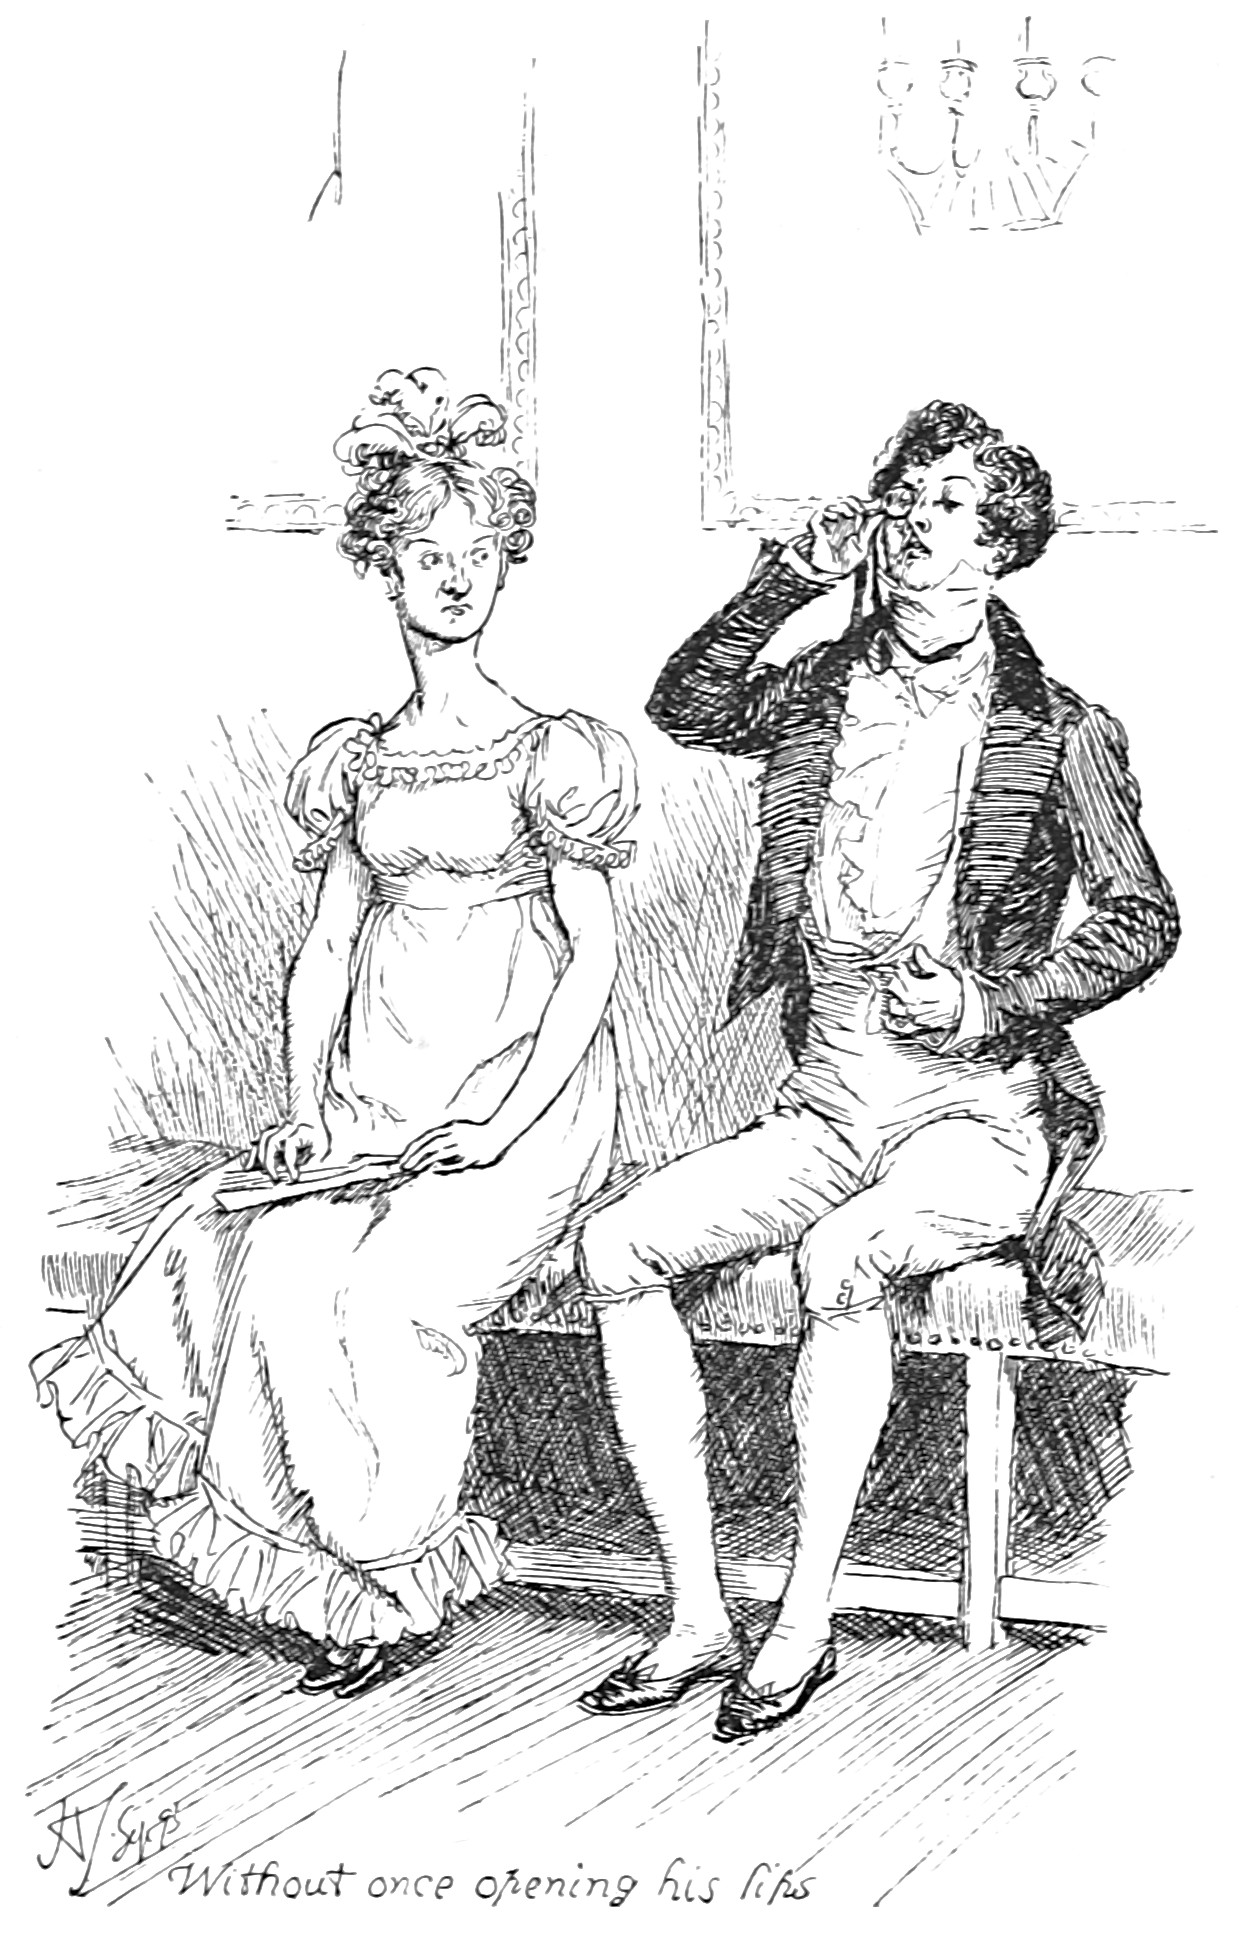
\includegraphics[width=.7\linewidth]{5lips}
\captionlistentry{Without ever opening his lips}
\end{figure}

»Are you quite sure, ma'am? Is not there a little mistake?« said Jane. »I certainly saw Mr Darcy speaking to her.«

»Ay, because she asked him at last how he liked Netherfield, and he could not help answering her; but she said he seemed very angry at being spoke to.«

»Miss Bingley told me,« said Jane, »that he never speaks much unless among his intimate acquaintance. With \textit{them} he is remarkably agreeable.«

»I do not believe a word of it, my dear. If he had been so very agreeable, he would have talked to Mrs Long. But I can guess how it was; everybody says that he is eat up with pride, and I dare say he had heard somehow that Mrs Long does not keep a carriage, and had to come to the ball in a hack chaise.«

»I do not mind his not talking to Mrs Long,« said Miss Lucas, »but I wish he had danced with Eliza.«

»Another time, Lizzy,« said her mother, »I would not dance with \textit{him}, if I were you.«

»I believe, ma'am, I may safely promise you \textit{never} to dance with him.«

»His pride,« said Miss Lucas, »does not offend \textit{me} so much as pride often does, because there is an excuse for it. One cannot wonder that so very fine a young man, with family, fortune, everything in his favour, should think highly of himself. If I may so express it, he has a \textit{right} to be proud.«

»That is very true,« replied Elizabeth, »and I could easily forgive \textit{his} pride, if he had not mortified \textit{mine}.«

»Pride,« observed Mary, who piqued herself upon the solidity of her reflections, »is a very common failing, I believe. By all that I have ever read, I am convinced that it is very common indeed; that human nature is particularly prone to it, and that there are very few of us who do not cherish a feeling of self-complacency on the score of some quality or other, real or imaginary. Vanity and pride are different things, though the words are often used synonymously. A person may be proud without being vain. Pride relates more to our opinion of ourselves; vanity to what we would have others think of us.«

»If I were as rich as Mr Darcy,« cried a young Lucas, who came with his sisters, »I should not care how proud I was. I would keep a pack of foxhounds, and drink a bottle of wine every day.«

»Then you would drink a great deal more than you ought,« said Mrs Bennet; »and if I were to see you at it, I should take away your bottle directly.«

The boy protested that she should not; she continued to declare that she would; and the argument ended only with the visit.

\begin{figure}[b!]
\centering
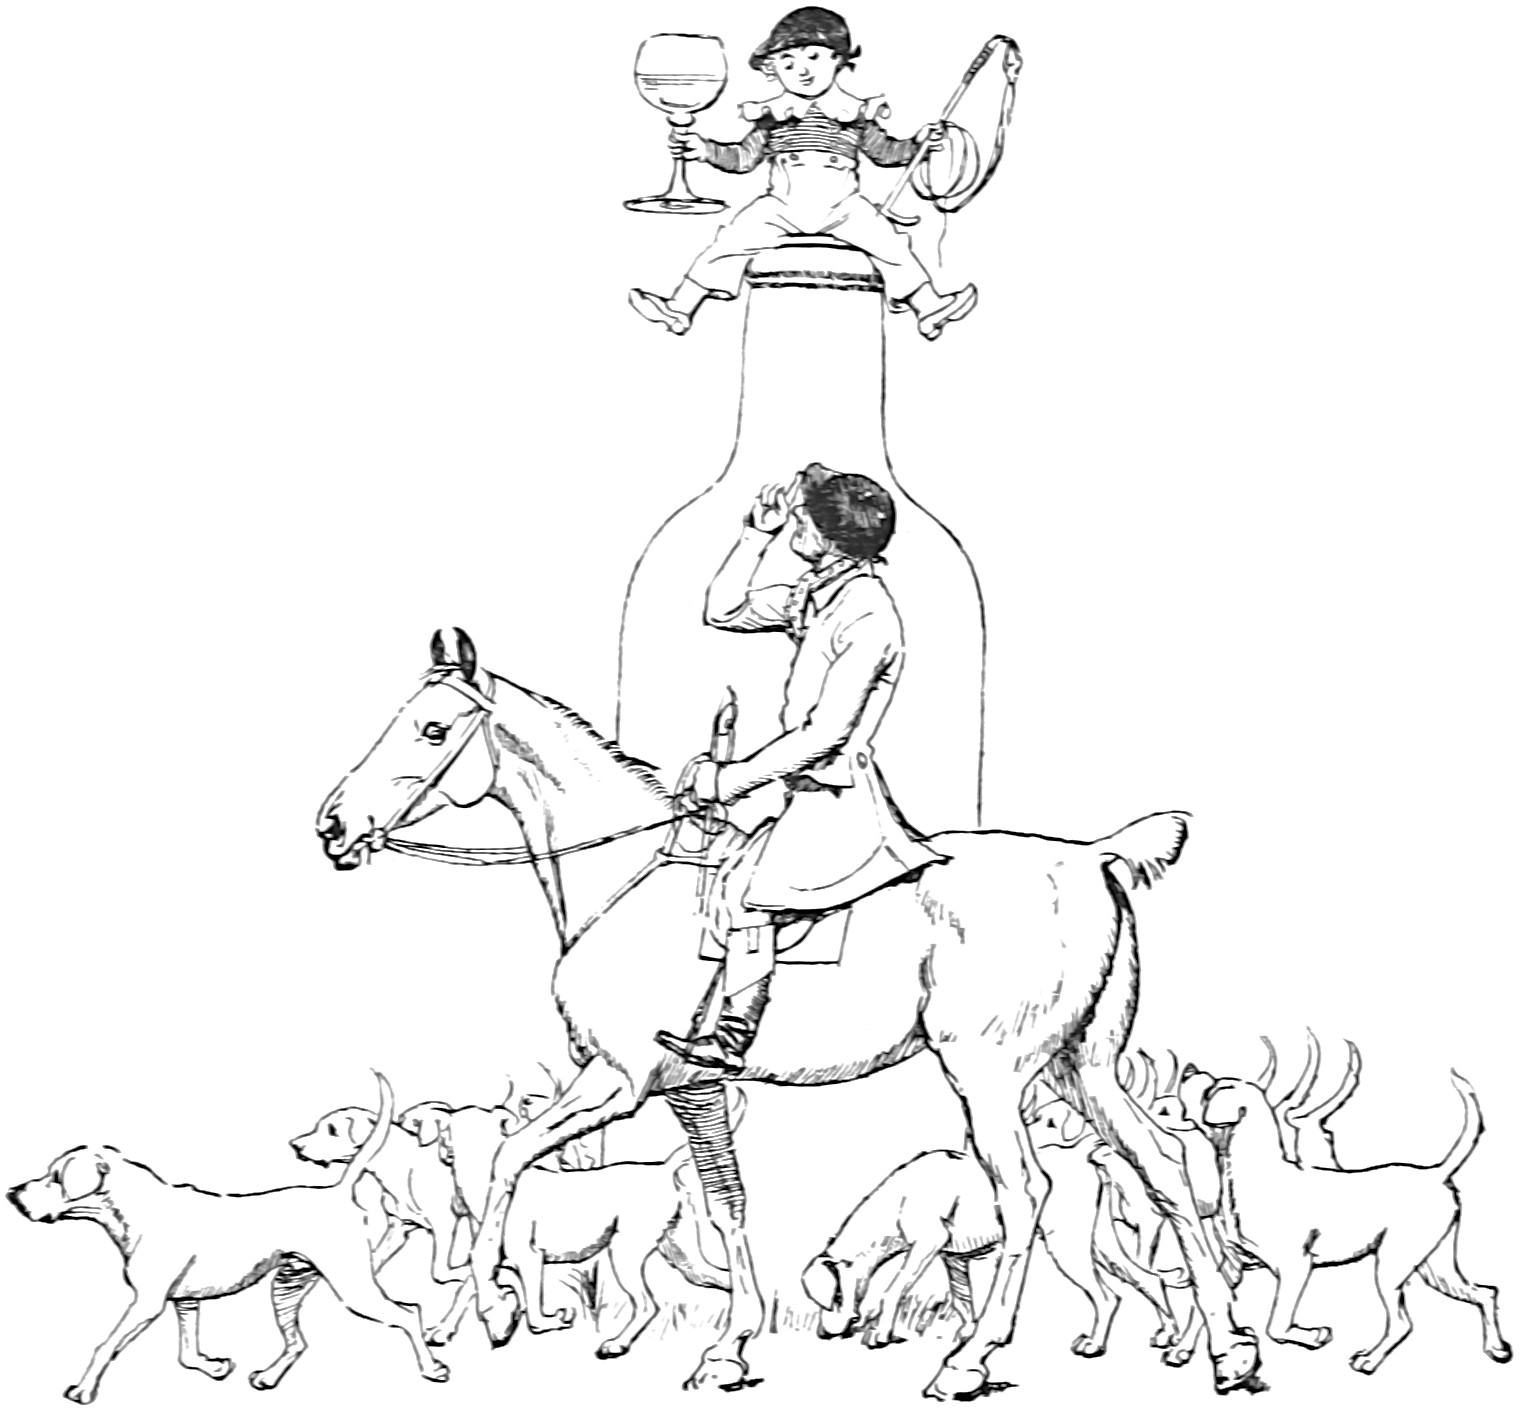
\includegraphics[width=.6\linewidth]{5bottle}
\captionlistentry{Tailpiece to Chapter \thechapter}
\end{figure}